%!TEX program = xelatex
%!TEX root = 
%!TEX option = 
\documentclass[11pt,letterpaper]{article} 
\usepackage[top=0.5in,bottom=0.5in,left=0.75in,right=0.75in]{geometry} 
\usepackage[CJKbookmarks]{hyperref}
\usepackage{xeCJK} 
\setCJKmainfont{FandolSong}
\usepackage{amsmath,amssymb,esint} 
\allowdisplaybreaks[0]
\numberwithin{equation}{section} % 公式编号包含章节
\usepackage{bm} 
\usepackage{siunitx} 
\usepackage{graphicx} 
\DeclareSIUnit\gauss{G}
\usepackage{array} 
\usepackage{multirow} 
\usepackage{braket}
\usepackage{tikz}
\usepackage{color}
\usepackage{multicol}
% \usepackage{tkz-euclide}
% \usepackage{tikz-feynman}

\renewcommand*{\vec}[1]{\bm{#1}} 
\newcommand{\dif}{\mathrm d}
\newcommand\mi{\mathrm{i}}
\newcommand\e{\mathrm{e}} 
\newcommand{\intf}[2][p]{\ensuremath{\int\frac{\dif^{#2}#1}{(2\pi)^{#2}}}\,} 
% Fourier integral
\DeclareMathOperator{\Diag}{Diag}

\DeclareMathOperator{\Hc}{H.c.}
\newcommand{\spind}{\ensuremath{\downarrow}}
\newcommand{\spinu}{\ensuremath{\uparrow}}

\begin{document}
\title{Note on Condensed matter}
\author{吕铭 Lyu Ming}
\maketitle
\begin{multicols}{2}
\tableofcontents
\end{multicols}
\section{Drude model and Sommerfeld model}
\label{sec:drude_model_and_sommerfeld_model}
A classical model, neglecting electron-electron interactions and most quantum
effects. 
\begin{itemize}
	\item Free carriers (e.g. electrons) and ``collision'' rate $1/\tau$
	\item Local equilibrium after the ``collision''
		\begin{itemize}
			\item Drude: Maxwell distribution
			\item Sommerfeld: Fermi-Dirac distribution
		\end{itemize}
\end{itemize}

The classical equation of motion gives DC conductivity and Hall effect: 
\begin{align}
	& m\dot{\vec v} = 0 = q\vec E - \frac{m\vec v}{\tau}
	&&\Leftrightarrow&&
	\vec j = qn\vec v = \frac{nq^2\tau}{m}\vec E = \sigma\vec E \\
	& m\vec v = 0 = q(\vec E + \vec \times \vec B) - \frac{m\vec v}{\tau}
	&&\Leftrightarrow&&
	\vec E = \frac{m}{nq^2\tau}\vec j - \frac{\vec j\times\vec B}{nq}
\end{align}

AC conductivity: 
\begin{align}
	&-\mi\omega m\vec v = q\vec E - \frac{m\vec v}{\tau}
	&&\Leftrightarrow&&
	\vec j = \frac{nq^2\tau}{m}\frac{1}{1-\mi\omega\tau}\vec E
\end{align}
gives complex conductivity, with in-phase dissipated part (real part) and
out-of-phase inductive part (imaginary part)
\subsection{Plasma frequency}
\label{sub:plasma_frequency}
AC field produce net surface charge and result in a frequency dependent
permittivity $E_{\mbox{in}} = E_{\mbox{out}}/\epsilon(\omega)$, with
\begin{equation}
	\epsilon(\omega) = 1 + \frac{\mi\sigma}{\omega\epsilon_0} 
	= 1 - \frac{nq^2\tau^2}{m\epsilon_0(1+\omega^2\tau^2)} +
	\mi\frac{nq^2\tau}{m\omega\epsilon(1+\omega^2\tau^2)}
\end{equation}
In the limit $\omega\tau \gg 1$, 
\begin{equation}
	\epsilon(\omega) \approx 1- \frac{nq^2}{m\epsilon_0+\omega^2} 
	\equiv 1- \frac{\omega_p^2}{\omega^2}
\end{equation}
with the \textbf{plasma frequency} $\omega_p = \sqrt{nq^2/m\epsilon_0}$. 
In good metal plasma frequency is in the ultraviolet. Here the metal becomes
more transparent instead of absorbing or reflecting E-M radiation.

\subsection{Heat current carried by charge carriers}
\label{sub:heat_current_carried_by_charge_carriers}
Average energy carried by the charge carrier gives the heat conductivity: 
\begin{equation}
	\vec j_Q = -n\langle v_x^2\rangle \tau \frac{\dif\varepsilon}{\dif T}\nabla T
\end{equation}
with $v_x$ meaning velocity along direction of $\nabla T$
\begin{center}
\begin{tabular}{c|cc}
                              & Drude model        & Sommerfeld model \\\hline
$\frac12\langle v_x^2\rangle$ & $\frac 12 k_BT$    & $\frac 13 E_F$ \\
$\dif\varepsilon/\dif T$      & $\frac 32 k_B$     & $\frac{\pi^2}2k_B^2T/E_F$ \\
product                       & $\frac 34 k_B^2 T$ &
$\frac{\pi^2}{6}k_B^2T$\\\hline
\end{tabular}
\end{center}

\section{Structure of crystal}
\label{sec:structure_of_crystal}
Gas and liquid fully respect the translational, reflectional and rotational
symmetry of space in their \emph{time-averaged structure}. Crystal breaks
both rotational and translational symmetries of space from continuous to
discrete, and has \emph{Long-range order}. 

\subsection{Classification}
\label{sub:classification}
\begin{itemize}
	\item 1-D crystals 
		\begin{itemize}
			\item 1 Bravais lattices
			\item 2 crystal symmetries: with(out) inversion symmetry
		\end{itemize}
	\item 2-D crystals 
		\begin{itemize}
			\item 5 Bravais lattices: minimum symmetry, rectangular, rhombic,
				square, hexagonal.
		\end{itemize}
	\item 3-D crystals: 
		\begin{itemize}
			\item 14 Bravais lattices: simple cubic, body centered cubic
				(BCC), face centered cubic (FCC)...
		\end{itemize}
\end{itemize}
\subsection{Observation (scattering)}
\label{sub:observation}
Real-space pictures: electron microscope, STM or X-ray microscope, etc. But
most widely-used is X-ray scattering (can also scatter neutron, electron,
atom, ion, ...). 

To scatter from a cell at $\vec R$, the scattering wave
\begin{align}
	\psi_s(\vec r) &\sim \frac{f}{|\vec r - \vec R|}\sum_{\vec R}\exp \left[
	\mi\vec k_i\cdot\vec R + \vec k_f\cdot(\vec r - \vec R)\right] \\
	&\approx \frac{\e^{\mi\vec k_f\cdot\vec r}}{|\vec r|}\sum_{\vec R} 
	f\e^{\mi\vec q\cdot\vec R}
	= \frac{\e^{\mi\vec k_f\cdot\vec r}}{|\vec r|}\int\dif\vec R \, \rho\e^{\mi
	\vec q \cdot\vec R}
\end{align}
with $\vec q = \vec k_i - \vec k_f$ the momentum transfer. So the amplitude 
\begin{equation}
	I = |\psi_s|^2 \sim \frac 1{r^2}\int\dif\vec R\,\e^{\mi\vec q \cdot\vec R} 
	\int\dif\vec R_2\,\rho(\vec R_2)\rho(\vec R_2+\vec R)
\end{equation}
is proportional to the Fourier transform of density-density correlation. 
\begin{itemize}
	\item In liquid, there's small peak showing typical distance between
		atoms
	\item In solid, $\delta$ functions in $\vec q=\vec G$ (``Bragg peaks'') with
		diffuse scattering from defects. \\
		$\vec G$: reciprocal lattice
		\begin{itemize}
			\item Finite crystals: $N = L\times L\times L$ \\
				$I\sim N^2$, $|\Delta q| \sim 1/L$, ``volume'' of the Bragg
				peak $\sim N$
			\item Diffuse scattering: $\rho(\vec r) = \rho_0(\vec r) + \delta
				\rho(\vec r, t)$\\
				$I\sim \sqrt{N}$
		\end{itemize}
\end{itemize}

\section{non-interacting Electrons and bands}
\label{sec:non_interacting_electrons}
First approximation: \emph{non-interacting electrons} in a perfect crystal;
treats electron-electron and electron-ion interactions only on average
(``mean-field'')
\begin{itemize}
  \item Discrete translational symmetry $\Rightarrow$ Bloch form gives 
	  ``crystal momentum'' $\vec q$ in the first Brillouin zone (FBZ). 
  \item Nearly free electron model
	  \begin{equation}
		  \psi_{n, \vec q}(\vec r) = \sum_{\vec G} \e^{\mi(\vec G+\vec
		  q)\cdot\vec r} \hat u_{n,\vec q}(\vec G)
	  \end{equation}
  \item Tight binding model
	  \begin{equation}
		  H = \sum_{\vec R, n}\epsilon^{(0)}_{\vec R, n} 
		  \hat c_{\vec R, n}^\dagger \hat c_{\vec R, n}
		  + \sum_{(\vec R, n)\neq (\vec R', n')} t_{\vec R, \vec R', n, n'}
		  \hat c_{\vec R', n'}^\dagger \hat c_{\vec R, n}
	  \end{equation}
  \item Band insulator: $E_F$ in a band gap. 
	  \begin{itemize}
	    \item For large gap, electron-electron/phonon interactions does not
			change much qualitatively
	  \end{itemize}
  \item Semiconductors\\
	  ``Dope'' a band insulator: to put some electrons in
	  the conduction band(s) and/or some holes in the valence band(s): 
	  \begin{itemize}
	    \item ``Intrinsic'' Semiconductors: doped by thermal excitations,
			especially in narrow-gap semiconductors
		\item Optically: Excite carriers by photons
		\item Gating: Thin sample, put large enough voltage and draw in
			carriers electrostatically
		\item Chemically: Put in other element from different columns of
			periodic table
			\begin{itemize}
			  \item ``n-type'', negative charge, carriers in conduction band
			  \item ``p-type'', positive charge, holes in valence band
			\end{itemize}
	  \end{itemize}
  \item Metals: In the non-interacting electron approximation, electron per
	  unit cell is not even or bans has overlap near $E_F$\\
	  Electron-electron interactions may open gaps at low $T$: 
	  \begin{itemize}
	    \item Superconductivity
		\item Charge-density wave (CDW)
		\item Spin-density wave (SDW)
		\item Mott insulator
	  \end{itemize}
\end{itemize}

Topology of FBZ
\begin{itemize}
  \item 1D, a circle
  \item 2D, a torus
  \item 3D, a ``3-torus''
\end{itemize}


\subsection{Single-particle Bloch states}
\label{sub:single_particle_bloch_states}
\begin{center}
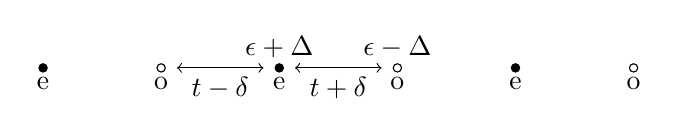
\begin{tikzpicture}
	\foreach \e in {0, 2, 4}
	\filldraw (1.5*\e, 0) circle (1.5pt) node[below]{e};
	\foreach \o in {1, 3, 5}
	\draw (1.5*\o, 0) circle (1.5pt) node[below]{o};
	\draw (3, 0) node[above]{$\epsilon+\Delta$}
		(4.5, 0) node[above]{$\epsilon-\Delta$};
	\def \s{0.2}
	\def \h{0}
	\draw[<->](3+\s, \h) -- node[below]{$t+\delta$} (4.5-\s, \h);
	\draw[<->](1.5+\s, \h) -- node[below]{$t-\delta$} (3-\s, \h);
\end{tikzpicture}
\end{center}
For given momentum $q$, this gives a $2\times 2$ Hamiltonian, written in
terms of $H_q = \epsilon + \vec h_q\cdot\vec\sigma$

Topology of a band: the topological properties of the continuous mapping FBZ
$\mapsto$ ``Bloch sphere''
\begin{itemize}
  \item 1D, circle $\mapsto$ circle, no topological special cases, but add
	  symmetry
	  \begin{itemize}
		  \item[:] $\Delta=0$, $\vec h_q$ on $x-y$ plane, there's topological
			distinct ``winding number''
			\begin{itemize}
			  \item $|t+\delta|>|t-\delta|$: winding number $=0$
			  \item $|t+\delta|<|t-\delta|$: winding number $=\pm 1$
			  \item Topological transition at $\delta=0$: gap closes at
				  $q=\pi/2a$ (edge of FBZ), where $\vec h_q = 0$
			\end{itemize}
	  \end{itemize}
\end{itemize}

\subsection{Edge states}
\label{sub:edge_states}
Topological insulators often have edge states with energies in the band gap.

For example 1D Kitaev model, the Majorana fermions, arose in superconductors,
are forced to be there by particle-hole symmetry.

\subsection{Direct measurement of bands}
\label{sub:direct_measurement_of_bans}
ARPES: Angle-Resolved Photo-Emission Spectroscopy

Scatter electrons by photons from a clean, flat surface. With known $\vec
q_{\mathrm{in}}, \epsilon_{\mathrm{in}}$, $\epsilon_{\mathrm{out}}, 
\vec q_{\mathrm{out}}$, and the scattering conservs $\vec q_\parallel$ to
surface, we can learn $\epsilon_n(\vec q)$ of occupied bands. Best for
quasi-2D materials (like hight-$T_c$ superconductors) and surface states
(like topological insulators).

To get unoccupied bands: Inverse photo-emission (under development).

\section{Density of states (DOS) of electrons in a crystal}
\label{sec:density_of_states_dos_of_electrons_in_a_crystal}
\begin{itemize}
	\item Number of quantum states $=$ one per ``volume'' $h^d =
		(2\pi\hbar)^d$ in $\vec r$-$\vec p$ space $=$ one per $(2\pi)^d$ in
		$\vec r$-$\vec k$ space
		\begin{equation}
			g(\epsilon) = \sum_{n\mbox{bands}} \frac{1}{(2\pi)^d}
			\int_{\mbox{FBZ}}\dif\vec k\,\delta(\epsilon - \epsilon_n(\vec
			k))
		\end{equation}
\end{itemize}

\subsection{van Hore singularities}
\label{sub:van Hore singularities}
\begin{itemize}
  \item At the edge of a band, $\dif\epsilon_n(\vec k)/\dif\vec k = \vec 0$
	  \begin{align} &|\epsilon(\vec k) -\epsilon_m|\sim k^2 \\
					&k\sim\sqrt{|\epsilon-\epsilon_m|} \\ &\mbox{``volume''
		  or No. of states} \sim |\epsilon - \epsilon_m|^{d/2} \\
	  &\mbox{DOS}\sim |\epsilon - \epsilon_m|^{(d-2)/2} 
	  \end{align}
	  \begin{itemize}
		  \item Quasi-1D(2D): much stronger hopping along one(two)
			  direction(s)
	  \end{itemize}
  \item At saddle points ?TBD?
	  \begin{itemize}
		  \item 3D: $(g-g_s)\sim\sqrt{\epsilon - \epsilon_s}$
		  \item 2D: $g\sim|\log|\epsilon -\epsilon_s||$
	  \end{itemize}
\end{itemize}
$g(E_F)$ is important for the low-$T$ properties of metals.

\subsection{Pauli para-magnetism}
\label{sub:pauli_paramagnetism}
Spin energy $E = \mu_B \vec H\cdot\vec\sigma$, which gives different Fermi
surface for different spins, and result in polarization (to the 1st order): 
\begin{equation}
	M \approx g(E_F)\mu_B^2 H; \qquad 
	\chi \equiv \frac{\dif M}{\dif H} = g(E_F)\mu_B^2
\end{equation}

Interactions between the spins can make big changes: magnetism and magnetic
ordering, or gaps opening suppressing this

\subsection[Low T electronic specific heat of metal]{Low $T$ electronic specific heat of metal}
\label{sub:low_t_electronic_specific_heat_of_metal}
\begin{align}
	u(T) &= \int\dif\epsilon\, \epsilon g(\epsilon)f\left(
	\frac{\epsilon - \mu(T)}{k_B T}\right) \\
	&\approx u(T=0) + \frac{\pi^2}{6}(k_BT)^2g(E_F) + 
	\mathcal O\left(\frac{k_BT}{E_F}\right)^3 \\
	c_{\mbox{el}} &= \frac{\dif u}{\dif T} = \frac{\pi^2}{3} k_B^2 T g(E_F)
\end{align}

Other main contribution to specific heat of a crystal: phonons. $c_p\sim T^2$
in 3D. Other effects due to defects can also give a linear-in-$T$ specific
heat, even in insulators. 

\section{Semi-classical dynamics of electrons in bands}
\label{sec:semi_classical_dynamics_of_electrons_in_bands}
Note the group velocity and dynamics of momentum: 
\begin{equation}
	\vec v(\vec q_0) = \frac 1\hbar \nabla_{\vec q}\epsilon_n |_{\vec q_0};
	\qquad
	F = \hbar\frac{\dif \vec q}{\dif t}
\end{equation}

Semi-classical dynamics: 
\begin{align}
	\frac{\dif \vec r}{\dif t} &= \vec v = \frac 1\hbar \nabla_{\vec
	q}\epsilon_n(\vec q) \\
	\frac{\dif \vec q}{\dif t} &= -\frac{e}{\hbar} (\vec E + \vec v\times
	\vec B)
\end{align}

For electrons at the top of a band $\epsilon_n = \hbar q^2/2m$ with $m<0$,
$-e/m = e/|m|$ is the same as positive mass and positive charge (holes). 

\subsection{Bloch oscillations}
\label{sub:bloch_oscillations}
Electron in band + uniform $\vec E$ field. $\vec q$ steadily ``increases''
but just winds around FBZ, with oscillations of velocity and position. 
\begin{itemize}
  \item The phenomenon can be observed for atoms in optical lattice
  \item For electrons in crystals it's difficult: need very clean + low $T$ +
	  weak coupling to phonons
\end{itemize}

\subsection{Landau levels in a band}
\label{sub:landau_levels_in_a_band}
The magnetic field does no work $\hbar\dot{\vec{q}} = e\vec B\times\vec v$, so
the particle follows ``contour'' of constant $\epsilon_n$ (e.g. follows Fermi surface). 
\begin{itemize}
  \item ``Open orbits'' do not close, so are not quantized in Landau levels,
	  and do not contribute to the Hall voltage. 
  \item ``closed orbits'' are quantized: $\Delta \epsilon = \hbar \omega_c$. 
	  The period 
	  \begin{equation}
		  T = \frac{2\pi}{\omega_c} = \oint\frac{|\dif\vec q|}{|\dot{\vec{q}}|}
		  = \frac{\hbar}{e B}\oint\frac{|\dif\vec q|}{|\vec v_\perp|}
		  = \frac{\hbar^2}{eB}\oint|\dif \vec q|\left|\frac{\dif\vec
		  q}{\dif\epsilon}\right| 
		  = \frac{\hbar^2}{eB}\frac{\dif A_q}{\dif\epsilon}
	  \end{equation}
	  which gives quantization of ``area'' in $\vec q$ space and \textbf{flux
	  quanta} from $\Delta \epsilon = \hbar\omega_c$
	  \begin{equation}
		  \Delta A_q = 2\pi\frac{eB}{\hbar} = \frac{B}{\Phi_0} 
		  \mbox{~~~with~~~}
		  \Phi_0 = \frac he
	  \end{equation}
	  \begin{itemize}
	    \item Motion $\parallel \vec B$ remains ``free'' and gives 1D-like
			van Hove singularity. 
		\item Number of states per Landau level: $D = \Phi/\Phi_0$
		\item Number of occupied Landau levels: $\nu = \Phi_0 A_q/B$
	  \end{itemize}
\end{itemize}

\subsubsection{Shubnikov-de Hass van Alphen oscillations}
\label{ssub:Shubnikov-de Hass van Alphen oscillations}
We get peaks DOS at $E_F$ periodically in $1/B$. Can be seen in specific
heat, resistivity and most qualities.
\begin{itemize}
  \item Low $T$: $f(\epsilon)$ is sharp compared to Landau-level spacing
  \item Clean material: To complete orbits before scattering
\end{itemize}

If there are more than one pieces of Fermi surface, get sum of contributions
each with its period in $1/B$: One way to measuring Fermi surface shape. 

\section{Lattice vibrations: phonons}
\label{sec:lattice_vibrations_phonons}
Nuclei are heavy: at low $T$ in most crystals, a classical, harmonic
approximation is a good first approximation (except hydrogen, helium).

For crystals with $N$ atoms per unit cell in $d$ dimension, there are $dN$
modes at each $\vec q$
\begin{itemize}
  \item Acoustic mode: longitudinal sound with $\hat \epsilon$ closer to
	  $\parallel \vec q$; transverse sound with $\hat epsilon$ closer to
	  $\perp \vec q$. \emph{Usually} $c_l > c_t$, crystal is ``stiffer'' to
	  compression than to shear. 
  \item Optic mode: with more than 1 atom per unit cell, has $q=0$
	  vibrations. In ionic photon's $\vec E$ couples strongly to optic
	  phonons, because of large electric dipole moment. See optic phonons as
	  inelastic light scattering. 
\end{itemize}

\subsection{Heat capacity due to phonons}
\label{sub:heat_capacity_due_to_phonons}
\begin{itemize}
	\item Classical regime $k_BT \gg \hbar \omega_n(\vec q)$, the heat capacity
	\begin{equation}
		C_{\mbox{phonon}} = 3k_B N_{\mbox{nuclei}} + \mbox{anharmonic terms}
	\end{equation}
	Interpreted as $3k_B$ per atom or $k_B$ per oscillator mode. 
	\item At low $T$ in 3 dimension
		\begin{equation}
			C_{\mbox{phonon}} \sim k_B N \left(\frac T{\theta_D}\right)^3
		\end{equation}
		Only acoustic phonons with $\hbar c|\vec q|\lesssim k_BT$
		contribute. 
\end{itemize}
Typically heat capacity of a metal $C\sim aT + bT^3$ with 1st term the
electron kinetic energy and 2nd term phonons.

\subsection{Structural instability of a crystal}
\label{sub:structural_instability_of_a_crystal}
\begin{itemize}
	\item A sound speed $\to 0$: unit cell disorts (usually to lower symmetry
		at lower $T$) 
	\item A phonon mode's $\omega(\vec q)\to 0$ at some $\vec q \neq 0$
		\begin{itemize}
		  \item At $\vec q = \vec G/n$: crystal distorts to have a larger
			  unit cell
		  \item At irrational fraction of $\vec G$: ``incommensurate
			  crystal'', no unit celll any more
		\end{itemize}
\end{itemize}
These structural transitions can all be ciewed as a type of Bose condensate,
but total distortion is limited by anharmonicities. 

\subsubsection{Peierls instability}
\label{ssub:Peierls instability}
A 1D equally spaced chain with one electron per ion is unstable. Distort
phonon $k = 2k_F$: 
\begin{enumerate}
	\item Coupling between $\epsilon(k)$ and $\epsilon(k-2k_F)$ gives energy
		shift 
		\begin{equation}
			\Delta\epsilon\sim -\frac{A^2}{|\epsilon_0(k-2k_F)-\epsilon(k)|}
			\sim -\frac{A^2}{\big||k|-|k_F|\big|\hbar v_F}
		\end{equation}
	\item Energy shift over all states in FBZ (cut off $\Omega\sim A$ 
		\begin{equation}
			\Delta E\sim -A^2 \left| \log \left( \frac{Aa}{\hbar v_F} \right) \right|
		\end{equation}
	\item Elestic energy $\sim A^2$. The band energy shift dominants,
		therefore there's a minimum at $A>0$. 
\end{enumerate}
This illustrates the much more general phenomenon that Fermi surfaces in
metals can be unstable to anything that opens a gap (superconducting being
another example). 

Treating the phonons fully \emph{quantum} means this instability may
\textbf{not happen} when it is very weak. 

\section{Electron-electron interactions}
\label{sec:electron_electron_interactions}
\subsection{Hubbard model}
\label{sub:hubbard_model}
To capture short-range part of electron-electron interactions within one
band. The ``simplest'' version: a one-band tight-binding model with on-site
electron-electron repulsion: 
\begin{equation}\label{eq:habbard} 
	H = U\sum_i \hat n_{i\spind}\hat n_{i\spinu} - t\sum_{\langle i, j\rangle,
	\sigma}\left( \hat c_{i, \sigma}^\dagger \hat c_{j,\sigma} + 
	\hat c_{j, \sigma}^\dagger \hat c_{i,\sigma}\right)
\end{equation}
Hubbard model is usually appropriate for compounds with one band crossing teh
Fermi energy. 

\subsubsection{Mott insulator}
\label{ssub:Mott insulator}
For $U\gg t$ in Hubbard model, ground state can have one electron per site so
band is only half-full. For $t=0$ (atomic limit) ground state for $N$ sites
is $2^N$-fold degenerate ($\spinu$ and $\spind$ spins). 

In grand canonical ensemble, ground state of $H-\mu N$ is\\
\begin{minipage}[b]{0.5\linewidth}
	\begin{center}
	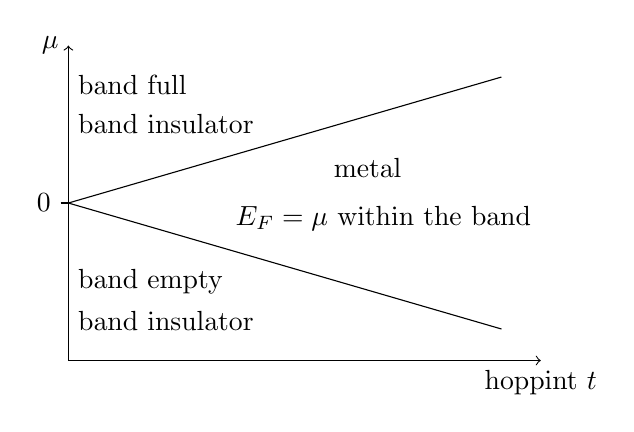
\begin{tikzpicture}
		\draw[->] (0,0)--(6,0) node[below]{hoppint $t$};
		\draw[->] (0,0)--(0,4) node[left]{$\mu$};

		\draw (-0.1,2)node[left]{$0$}--(0,2);
		\draw (0,3.5)node[right]{band full}
			(0,3)node[right]{band insulator};		
		\draw (0,2)--(5.5,3.6);
		\draw (2,1.8)node[right]{$E_F=\mu$ within the band}
			(3.8, 2.2) node[above]{metal};
		\draw (0,2)--(5.5,0.4);
		\draw (0,1)node[right]{band empty}
			(0,0.5)node[right]{band insulator};		
	\end{tikzpicture}\\
		$U=0$
	\end{center}
\end{minipage}%
\begin{minipage}[b]{0.5\linewidth}
	\begin{center}
	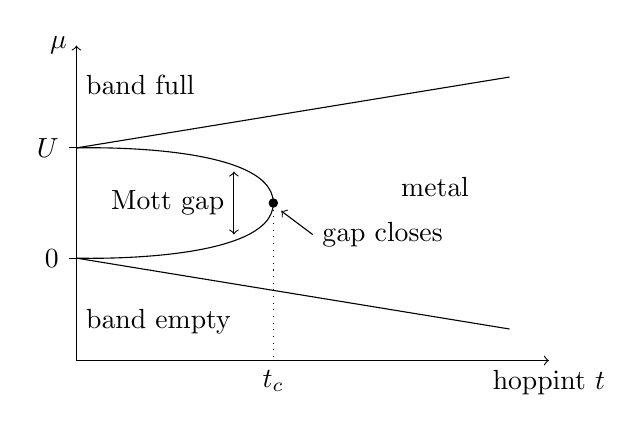
\begin{tikzpicture}
		\draw[->] (0,0)--(6,0) node[below]{hoppint $t$};
		\draw[->] (0,0)--(0,4) node[left]{$\mu$};

		\draw (0,3.5)node[right]{band full};
		\draw (0,2.7)--(5.5,3.6);
		\draw (-0.1,2.7)node[left]{$U$}--(0,2.7);

		\draw plot[smooth, tension=2] coordinates {(0,2.7) (2.5,2) (0,1.3)};
		\filldraw (2.5, 2) circle (1.5pt);
		\draw[<-] (2.6,1.9)--(3, 1.6)node[right]{gap closes};
		\draw[dotted] (2.5,2)--(2.5,0)node[below]{$t_c$};
		\draw (4,2.2)node[right]{metal};
		\draw[<->] (2, 2.4) -- node[left]{Mott gap} (2, 1.6);

		\draw (-0.1,1.3)node[left]{$0$}--(0,1.3);
		\draw (0,1.3)--(5.5,0.4);
		\draw (0,0.5)node[right]{band empty};
	\end{tikzpicture}\\
		$U>0$
	\end{center}
\end{minipage}
\begin{itemize}
  \item Mott insulator has $E_F$ in ``Mott gap'', and the band is half-filled
  \item For $t<t_c$, there's upper(lower) Hubbard band
  \item Many materials are Mott insulators due to strong electron-electron
	  interactions
  \item Mott insulator has a ``charge gap'' but not a ``spin gap''
\end{itemize}
Mott insulators and the Hubbard model are also realized with cold neutral
atoms in optical lattices. The neutral atoms don't have Coulomb interaction,
only ``contact'' interaction. Atoms can be either fermions or bosons, and may
have many spin (hyperfine) state. 

\textbf{Bose-Hubbard} model allows any numver of bosons on site: 
\begin{equation}
	H = \frac U2 \sum_i n_i(n_i - 1) - t\sum_{\langle i, j\rangle} \left( 
\hat c_i^\dagger \hat c_j + \hat c_j^\dagger \hat c_i\right)
\end{equation}
\begin{center}
  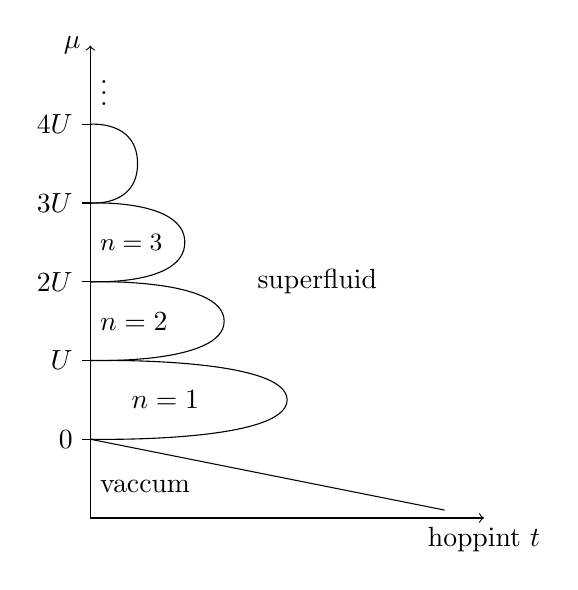
\begin{tikzpicture}
	\draw[->] (0,0)--(5,0) node[below]{hoppint $t$};
	\draw[->] (0,0)--(0,6) node[left]{$\mu$};

	\draw (-0.1,2)node[left]{$U$}--(0,2);
	\draw plot[smooth, tension=2] coordinates {(0,2) (2.5,1.5) (0,1)};
	\draw (0.4,1.5)node[right]{$n=1$};

	\draw (-0.1,3)node[left]{$2U$}--(0,3);
	\draw plot[smooth, tension=2] coordinates {(0,3) (1.7,2.5) (0,2)};
	\draw (0,2.5)node[right]{$n=2$};

	\draw (-0.1,4)node[left]{$3U$}--(0,4);
	\draw plot[smooth, tension=2] coordinates {(0,4) (1.2,3.5) (0,3)};
	\draw (0,3.5)node[right]{\small $n=3$};

	\draw (-0.1,5)node[left]{$4U$}--(0,5);
	\draw plot[smooth, tension=2] coordinates {(0,5) (0.6,4.5) (0,4)};

	\draw (0, 5.5)node[right]{$\vdots$};
	\draw (2,3)node[right]{superfluid};

	\draw (-0.1,1)node[left]{$0$}--(0,1);
	\draw (0,1)--(4.5,0.1);
	\draw (0,0.4)node[right]{vaccum};
  \end{tikzpicture}
\end{center}

\subsubsection{Magnetism}
\label{ssub:Magnetism}
Spin interactions in a Hubbard model ( Eq.~\ref{eq:habbard}). Simplest case:
2 electrons on two sites, 6 two-particle states: 
\begin{itemize}
	\item total spin zero: $\ket{2, 0}$, $\ket{0,2}$,
		$(\ket{\spinu,\spind}-\ket{\spind,\spinu})/\sqrt 2$
	\item total spin one: $\ket{\spinu,\spinu}$, $\ket{\spind, \spind}$
		$(\ket{\spinu,\spind}+\ket{\spind,\spinu})/\sqrt 2$
\end{itemize}
The ground state: 
\begin{itemize}
	\item $U=0$: 
		\begin{itemize}
		  \item single-particle $(\ket{\sigma,0}+\ket{0,\sigma})/\sqrt{2}$
			  with $\epsilon = -t$
		  \item Two-particle $(\ket{2,0}+\ket{0,2} +
			  \ket{\spinu,\spind}-\ket{\spind,\spinu})/2$ with $\epsilon=-2t$
		\end{itemize}
		Pauli exclusion produces anti-ferromagnetic spin corelations, which
		does not rely on interactions
	\item $t=0$: 4-fold degenerate ground state of $E=0$, the states
		$\ket{\spinu,\spind}$, $\ket{\spind,\spinu}$, $\ket{\spinu,\spinu}$,
		$\ket{\spind,\spind}$. 
	\item General $U$, $t$, total spin $S=1$ gives $E=0$, $S=0$ states: 
		\begin{equation}
			E = \frac U2\pm\sqrt{ \left( \frac U2 \right)^2 + 4t^2}
		\end{equation}
\end{itemize}

\textbf{Ferromagnetism} requires: 
\begin{itemize}
	\item Degenerate and partially filled orbitals (p, d, f... orbitals)
	\item Coulomb interaction: anti-symmetry space wave-function
\end{itemize}
From three-site Hubbard model:
\begin{itemize}
  \item $U=0$ single-particle eigenstates: 
	  \begin{itemize}
		  \item $l=0$, $(\ket A + \ket B + \ket C)/\sqrt 3$, $\epsilon=2t$
		  \item $l=1$, $(\ket A + w\ket B + w^*\ket C)/\sqrt 3$, $\epsilon=-t$
			  \footnote{$w=\exp (2\mi \pi/3)$}
		  \item $l=-1$, $(\ket A + w^*\ket B + w\ket C)/\sqrt 3$, $\epsilon=-t$
	  \end{itemize}
  \item Weak $U$, total $S$, $S_z$, $l$ can be good quantum number for two electron.
	  For $l=\pm1$ single-particle states:  
	  \begin{itemize}
	    \item Total $S=0$ states all have doubly-occupied sites, total
			$l=\pm2$ or $0$, 3 states, higher energy for $U>0$; 
		\item Total $S=1$ has no doubly-occupied sites, total $l=0$, 3 states
	  \end{itemize}
	  Total $S=1$ ground state for weak $U$
  \item Strong $U$, starting from single occupied with one $\spinu$, the
	  other $\spind$, and add hopping. Ground state $E=-2t$ is still total
	  $S=1$
\end{itemize}

\subsection{Spin models}
\label{sub:spin_models}
A spin $\vec S_i$ on each atom: 
\begin{equation}
	H_s = \sum_{\langle i, j\rangle} \vec S_i \overleftrightarrow J_{ij}\vec S_j
	+\sum_i \vec h_i\cdot\vec S_i
\end{equation}

\subsubsection{Heisenberg model}
\label{ssub:Heisenberg_model}
For spin-$1/2$, isotropic interactions: 
\begin{equation}
  H = \sum_{\langle i,j\rangle}J_{ij}\vec S_i\cdot\vec S_j
\end{equation}
\begin{itemize}
  \item If $J_{ij}<0$, ground state is ferromagnetic. Ground state $\sum S =
	  \sum S_z = N/2$
	\begin{itemize}
	  \item ``Spin waves'': Excited states with one spin flipped: 
		  \begin{equation}
			  \vec S_i\cdot\vec S_j = S_{iz}S_{jz} + \frac 12 \left( 
			  S_{i+}S_{j-}+S_{i-}S_{j+}\right)
		  \end{equation}
		  spin-flip is a ``hard-core'' boson. The wave $\omega(q)\sim q^2$
		  for small $q$
	\end{itemize}
	Most ferromagnets $J$ comes from Coulomb interaction + Pauli exclusion.
	Weaker but long-range ($\sim 1/t^3$) magnetic dipole interaction contributes
	at long length scale: \textbf{``shape anisotropy''} 
  \item Anti-ferromagnets: spins anti-align in ground state. 
	  \begin{itemize}
	    \item The Simplest case: two sub-lattices $\spinu, \spind$, doubles the
			unit cell and a new Bragg peak appear (\emph{magnetic Bragg peak}. 
		\item Spin-waves: $\omega(q)\sim q$ (Anderson, \~ 1952)
		\item Order parameter: $\vec S_A - \vec S_B$
		\item \textbf{Frustrated anti-ferromangets}: can't minimize energy of
			all interactions.  The Simplest example: 3 spins on a trangle: 
			\begin{center}
			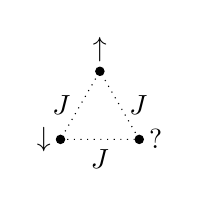
\begin{tikzpicture}
				\filldraw (-0.5, 0) circle (1.5pt) node[left]{$\spind$}
					(0.5, 0) circle (1.5pt) node[right]{?}
					(0, 1.73/2) circle (1.5pt) node[above]{$\spinu$};
				\draw[dotted] (-0.5,0)--node[below]{$J$}(0.5,0)--
					node[right]{$J$}(0,1.732/2)--node[left]{$J$}(-0.5,0);
			\end{tikzpicture}
			\end{center}
			is minimized by minimal total spin: $H=J/2 (\sum \vec S_i)^2 -
		J/2 (\sum \vec S_i^2)$. 
		\begin{itemize}
		  \item Kagome lattice: For spin configuration, there's no long range
			  order, no anti-ferromangets --- \textbf{spin liquid}.
		\end{itemize}
	\end{itemize}
\end{itemize}

\section{Superconductivity and superfluidity}
\label{sec:superconductivity_and_superfluidity}
\subsection{Phenomena}
\label{sub:phenomena}
\begin{itemize}
  \item Zero Ohmic resistivity: super currents that flow without dissipation
  \item Meissner effect: magnetic fields are either expelled from the material,
	  or confined to flux lines on vortices 
  \item Josephson effect
  \item ......
\end{itemize}

\subsection{Pairing and ground state}
\label{sub:pairing}
In some superconductors, such as high-$T_c$, the mechanism by which electrons
attract is still not known; in many superconductors it is known that
electron-phonon interactions produce the attraction. 

In the absence of a Fermi sea, two quantum particles with a \emph{weak} attraction
do always form a bound state in 1D and 2D, but not in 3D or higher; but in
the presence of a filled Fermi seam 2 fermions do bind. 

\begin{equation}
	H = \sum_{\vec q}\epsilon_{\vec q} (\hat n_{\vec q, \spinu} + \hat
	n_{\vec q, \spind})
\end{equation}
The interaction term:
\begin{align}
	U &= \sum_{\vec R}\sum_{\vec r} U(\vec r) \hat c_{\vec R ,\spinu}^\dagger \hat
	c_{\vec R ,\spinu}\hat c_{\vec R+\vec r,\spind}^\dagger\hat c_{\vec
	R+\vec r,\spind} \\
	&= \frac 1{2N}\sum_{\vec q_1 +\vec q_2 = \vec q_3 + \vec q_4} 
	\tilde U(\vec q_2 - \vec q_3) \hat c_{\vec q_1,\spinu}^\dagger
	\hat c_{\vec q_2,\spind}^\dagger \hat c_{\vec q_3, \spind}
	\hat c_{\vec q_4,\spinu}
\end{align}
The Cooper problem with $\tilde U(\vec q) = U < 0$ is constant, which
corresponds to $U(\vec r) = U\delta(\vec r)$

\subsubsection{Single particle pairing}
\label{ssub:Simgle particle pairing}
For coupling only above Fermi sea, the pairing of the form: 
\begin{equation}
	\ket{\psi} = \sum_{\vec q} a_{\vec q} c_{\vec q,\spinu}^\dagger
	c_{-\vec q, \spind}^\dagger \ket{\mbox{Fermi sea}}
\end{equation}
has binding energy $E \approx 2 E_F - 2(\Omega - E_F)\exp[2/Ug(E_F)]$. Note
that the result is non-purtubative in $U$. 

In general, weak attraction and filled Fermi sea give binding of Cooper
pairs. If $U(\vec q)$ is not always negative, the lowest energy Cooper pair
may be in some other ``pairing channel'' such as triplet, p-wave; or singlet,
d-wave (high-$T_c$ superconductors pair this way), so Cooper pairs are not
always s-wave, total spin $0$.  

\subsubsection{Full many-body BCS pairing}
\label{ssub:Full many-body BCS pairing}
\begin{align}
	H-\mu N &= \sum_{\vec q \sigma} (\epsilon_{\vec q} - \mu)
	\hat c_{\vec q,\sigma}^\dagger \hat c_{\vec q, \sigma} + 
	\frac 1{2N} \sum_{\vec k_1, \vec k_2, \vec q} \tilde U(\vec q)
	\hat c_{\vec k_1,\spinu}^\dagger \hat c_{\vec k_2+\vec q,\spind}^\dagger
	\hat c_{\vec k_2,\spind} \hat c_{\vec k_1+\vec q, \spinu} \\
	&= \sum_{\vec q \sigma} (\epsilon_{\vec q} - \mu)
	\hat c_{\vec q,\sigma}^\dagger \hat c_{\vec q, \sigma} + 
	\frac 1{2N} \sum_{\vec k, \vec q} \tilde U(\vec k - \vec q)
	\hat c_{\vec k,\spinu}^\dagger \hat c_{-\vec k,\spind}^\dagger
	\hat c_{\vec -q,\spind} \hat c_{\vec q, \spinu}
	+\mbox{``non-paired'' terms}
\end{align}
The BCS (variational) wavefunction is of the form: 
\begin{equation}
	\ket{\Psi_{\mathrm{BCS}}} = \prod_{\vec q} \left( \sin\theta_{\vec q} + 
	\cos\theta_{\vec q}\e^{\mi\phi_{\vec q}} \hat c_{\vec q,\spinu}^\dagger
	\hat c_{-\vec q,\spind}^\dagger\right)\ket{0}
\end{equation}
In this wavefunction $\langle \mbox{``non-paired terms''}\rangle = 0$ 
\begin{equation}
	\langle H -\mu N\rangle = \sum_{\vec q}\cos^2\theta_{\vec q}
	(\epsilon_{\vec q} - \mu) + \frac 1{2N}\sum_{\vec k, \vec q} 
	\tilde U(\vec k - \vec q) \e^{\mi(\phi_{\vec q} - \phi_{\vec k})}
	\cos\theta_{\vec k}\sin\theta_{\vec k}\cos\theta_{\vec q}\sin\theta_{\vec q}
\end{equation}
\begin{itemize}
	\item If $U(\vec q)<0$, for all $|\vec q|\le 2k_F$ minimum energy has
		$\phi_{\vec q} = \phi_{\vec k} = \mbox{const.}$: s-wave paring
		(most common)
	\item If $U((\vec q)>0$, for some $|\vec q|<2k_F$ minimum energy might
		have p-wave, d-wave, etc. 
\end{itemize}
For $\tilde U(\vec q) = U<0$, minimization of $\langle H-\mu N\rangle$ gives:
\begin{equation}
	\frac{\sin 2\theta_{\vec q}}{\cos 2\theta_{\vec q}} =
	\frac{\Delta}{\mu-\epsilon} 
	\qquad 
	\Delta = -\frac{U}{2N}\sum_{\vec q}\sin 2\theta_{\vec q}
\end{equation}
\begin{itemize}
  \item Far below $\epsilon_q = \epsilon_F$, $\theta_q\to 0$, electron present
  \item Far above $\epsilon_q = \epsilon_F$, $\theta_q\to 0$, electron absent
  \item At $\epsilon_q = \epsilon_F$, $\theta_q = \pi/4$, equal amplitude
  \item The occupation number $\langle \hat n_q\rangle = \cos^2\theta_q$
	  \begin{equation}
		  \langle\hat n_q\rangle = \frac 12 \left( 1 + \frac{\mu-\epsilon_q}
		  {\sqrt{\Delta^2+(\mu-\epsilon_q)^2}}\right)
	  \end{equation}
	  has $\sim\Delta$ width near ``Fermi surface'' and thus no sharp jump;
	  $\sim \big[\Delta/(\epsilon-\epsilon_F)\big]^2$ as $\epsilon \gg
	  \epsilon_F$, longer tails than Fermi-Dirac function
\end{itemize}

The ``gap'' $\Delta$ should satisfy the gap equation: 
\begin{equation}
  1 = \frac{|U|}{2N}\sum_{\vec q}\frac 1{\sqrt{\Delta^2 + (\mu-\epsilon_{\vec
  q}^2})} = |U|\int\dif\epsilon\,
	  \frac{g(\epsilon)}{\sqrt{\Delta^2-(\epsilon-\epsilon_F)^2}}
\end{equation}
\begin{itemize}
  \item Weak gap/weak coupling: 
	  \begin{equation}
		  \Delta \sim \Omega\e^{-1/g(\epsilon_F)|U|}
	  \end{equation}
	  with $\Omega \sim \hbar\omega_{\mbox{phonon}}$ being the cut off
  \item $\Delta$ and pairing mean field: 
	  \begin{equation}
		  \Delta(\vec q) \equiv \frac 1N \sum_{\vec k} \tilde U(\vec k-\vec
			  q)\langle \hat c_{-\vec k,\spind} \hat c_{\vec k, \spinu}\rangle
	  \end{equation}
	  is consistent with the definition before. 
\end{itemize}

\subsection{Excitations}
\label{sub:excitations}
In the mean field approximation, for states at $\vec q, \spinu$, $-\vec q,
\spind$: 
\begin{equation}
	(H-\mu N)_{\vec q} = (\epsilon_{\vec q} - \mu)(\hat n_{\vec q,\spinu} + 
	\hat n_{-\vec q, \spind}) - \Delta(\vec q)\hat c_{\vec q,\spinu}^\dagger
	\hat c_{-\vec q,\spind}^\dagger - \Delta^*(\vec q) \hat c_{-\vec q,\spind}
	\hat c_{\vec q, \spinu}
\end{equation}
whose eigenenergy is $E = \epsilon_q - \mu$ (2-fold), $E = (\epsilon_q-\mu)
\pm \sqrt{|\Delta(q)|^2+(\epsilon_q-\mu)^2}$, with ground state we get before
\begin{equation}
	(\sin\theta_q + \e^{\mi\phi_q}\cos\theta_q \hat c_{q,\spinu}^\dagger
	\hat c_{-q,\spind}^\dagger)\ket{0}
\end{equation}
And the self-consistant gap equation
\begin{equation}\label{eq:pari_gap_in_exci}
	\Delta(\vec q) = \e^{\mi\phi_{\vec q}}\sin 2\theta_{\vec q}\sqrt{
	|\Delta(\vec q)|^2+(\epsilon_{\vec q}-\mu)^2}
\end{equation}

Here $\ket 0$ means BCS ground state at other $\vec q$. The excitation can be
described by quasiparticles (\textbf{Bogoliubov rotation})
\begin{align}
	& \hat b_{\vec q, \spinu}^\dagger = \sin\theta_{\vec q}\hat c_{\vec q, \spinu}^\dagger
	-\e^{-\mi\phi_{\vec q}}\cos\theta_{\vec q}\hat c_{-\vec q,\spind} \\
	& \hat b_{-\vec q, \spind}^\dagger = \sin\theta_{\vec q}\hat c_{-\vec q,
	\spind}^\dagger	+\e^{-\mi\phi_{\vec q}}\cos\theta_{\vec q}\hat c_{\vec q,\spinu} 
\end{align}
so that 
\begin{equation}
	(H-\mu N)_{\vec q} = \sqrt{|\Delta(\vec q)|^2 + (\epsilon_{\vec q}
	-\mu)^2} \left( \hat b_{\vec q,\spinu}^\dagger\hat b_{\vec q,\spinu} + 
	\hat b_{-\vec q,\spind}^\dagger \hat b_{-\vec q,\spind}\right) + E_0
\end{equation}
\begin{itemize}
	\item The quasi-particle energy/excitation gap $E_{q} = \sqrt{|\Delta(\vec
		q)|^2 + (\epsilon_{\vec q} -\mu)^2} >|\Delta(\vec k_F)|$
	\item For $\Delta(\vec q) = \Delta = \mbox{const.}$, at $E=|\Delta|$, DOS
		of quasi-particles has 1D-like van Hove singularity. There're no states
		between $E = E_F \pm |\Delta|$ \textcolor{red}{gap vs condensate?}
		\begin{itemize}
		  \item This is seen in STM: no tunneling current when
			  $|eV|<|\Delta|$
		  \item Not the case for p-wave or d-wave: there's node for
			  $\Delta(\vec q)$
		\end{itemize}
\end{itemize}

\subsubsection{Finite temperature}
\label{ssub:Finite_temperature}
For excited states, $\langle c_{-\vec q,\spind} c_{\vec f,\spinu}\rangle =
\Delta/2E_{\vec q}$ (ground state, from Eq.~(\ref{eq:pari_gap_in_exci}), with
$E_{\vec q}$ the quasi-particle energy) $0$ (1 quasi-particle) or
$-\Delta/2E_{\vec q}$. So the Boltzmann average of $\langle c_{-\vec
q,\spind} c_{\vec f,\spinu}\rangle$ gives: 
\begin{equation}
	\Delta = \frac{|U|}{N}\sum_{\vec q}
	\frac{\e^{E_k/T}-\e^{-E_k/T}}{\e^{E_k/T}+2+\e^{E_k/T}}
	\frac{\Delta}{2E_k}
	\sim \Delta |U|g(\epsilon_F)\ln \left( \frac{\Omega}{\max (T,\Delta)} \right)
\end{equation}
\begin{itemize}
	\item For $T$ too high (roughly $T>\Delta(T=0)$), $\Delta=0$ is the only
		solution: phase transition $T_c$. Near $T_c$, $\Delta\sim\sqrt{T_c -
		T}$
\end{itemize}

\subsubsection{Total spin of pairs}
\label{ssub:Total_spin_of_pairs}
For pair of $\vec q$ and $-\vec q$, 
\begin{itemize}
	\item If $l$ is even ($\Delta(\vec q) = \Delta(-\vec q)$, s-wave and
		d-wave), $S=0$
	\item If $l$ is odd ($\Delta(\vec q) = -\Delta(-\vec q)$, p-wave),
		$S=1$\\
		This occurs for superfluid $^3$He and for electrons in some materials
\end{itemize}

\subsection{Superfluid wavefunction}
\label{sub:superfluid_wavefunction}
Phenomenally define the wavefunction $\Psi(\vec r, t) \sim \Delta(\vec r, t)$
with $\Psi(\vec r, t) = |\Psi(\vec r, t)|\e^{\mi\phi(\vec r, t)}$ and number
density of bosons $n = |\Psi|^2$
\begin{itemize}
  \item Number current: 
	  \begin{equation}\label{eq:sc_current}
		  \vec j_n = \frac{\hbar}{m^*}\Im \left[ \Psi^* \left( \nabla -
			  \mi\frac q\hbar \vec A \right) \Psi \right] 
			  = |\Psi|^2\frac\hbar{m^*} \left( \nabla\phi - \frac q\hbar \vec
				  A  \right) = n\vec v_s
	  \end{equation}
  \item London approximation: $|\Psi| = \mbox{const.}$ for $T\ll T_c$ which
	  leads to \textbf{London equations}
  \item Ginzburg-Landau equations allow variation in $|\Psi|$
\end{itemize}

\subsection{London equations and Meissner effect}
\label{sub:Meissner effect}
From Maxwell equation 
\begin{equation}
  \nabla\times\vec A = \vec B \qquad \nabla\times\vec B = \mu_0\vec j
\end{equation}
and equation of current Eq.~(\ref{eq:sc_current}), $\vec j = q\vec j_n$,
give London equation
\begin{equation}
	\nabla\times\vec j = -\frac{n q^2}{m^*}\vec B
	\mbox{~~~or~~~}
	\vec j = -\frac{nq^2}{m^*}\vec A
\end{equation}
The second form requires Coulomb gauge. This promises exponential decay of
$\vec B$ into the bulk. The penetration length: 
\begin{equation}\label{eq:penetration_length}
	\lambda = \sqrt{\frac{m^*}{\mu_0 n q^2}}
\end{equation}

\subsubsection[Critical field Hc]{Critical field $H_c$}
\label{ssub:critical_field}
The free energy of normal state $f_n(T)$ and superconductor state $f_s(T) +
H^2/2\mu$ give the critical field $H_c =
\sqrt{2\mu_0\big[f_n(T)-f_s(T)\big]}$: 1st order transition (vanishes
linearly at $T\to T_c$)
\begin{itemize}
  \item Type-I superconductors: the above happens
  \item Type-II superconductors have intermediate phase with vortices and
	  flux lines
\end{itemize}

\textbf{Shape and size effects}: for example long slab with normal field. 
\begin{center}
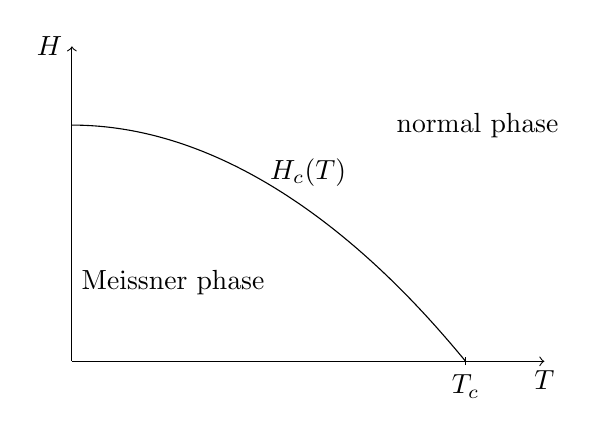
\begin{tikzpicture}
	\draw[->] (0,0)--(6,0) node[below]{$T$};
	\draw[->] (0,0)--(0,4) node[left]{$H$};

	\draw (0,3) parabola (5,0);
	\draw (3,2.1) node[above]{$H_c(T)$}
		(0,1)node[right]{Meissner phase}
		(4,3)node[right]{normal phase};
	\draw (5,-0.05) node[below]{$T_c$} -- (5,0.05);
\end{tikzpicture}\\
Phase diagram of type-I superconductor
\end{center}
\begin{itemize}
  \item For most superconductors, energy of currents and flux expulsion $\gg$
	  Zeeman energy, so coupling to electron spins can be ignored. Exceptions
	  like thin film or wires in parallel fields. 
\end{itemize}

\subsubsection{Flux quantization (Aharonor-Bohm effect)}
\label{ssub:flux_quantization}
For theck loop of superconductor ($d\gg\lambda$), around path inside
superconductor $\vec j = 0 = \nabla\phi - q\vec A/\hbar$. Wavefunction is
single valued, so $\oint\nabla\phi\cdot\dif\vec l = 2\pi k$ with $k\in\mathbb Z$
\begin{equation}\label{eq:phi0}
	\frac q\hbar\oint\vec A\cdot\dif\vec l = \frac q\hbar \Phi = 2\pi k
	\qquad 
	\Phi = k\Phi_0 = k\frac hq
\end{equation}
where $\Phi$ is magnetic flux through the loop, $\Phi_0$ is the quantum of
magnetic flux, and for superconductor $\Phi_0 = h/2e$ 

\subsubsection[supercurrent in E-field]{Supercurrent in $\vec E$-field}
\label{ssub:super_current}
Schr\"odinger equation of $\phi$
\begin{equation}
	\hbar\frac{\dif\phi(\vec r)}{\dif t} = -2eV(\vec r)
\end{equation}
Combining with Eq.~(\ref{eq:sc_current}) and $\vec A=0$, $\vec E = -\nabla
V$, we get $m\dot{\vec v}_s = 2e\vec E$ is free acceleration of the
supercurrent. This happens until $v_s$ gets high enough to produce
quasi-particles or vortices: ``critical current''. 

\subsubsection{Josephson junction}
\label{ssub:josephson_junction}
In a superconductor 1 (with phase $\phi_1$) -- insulator -- superconductor 2
(with phase $\phi_2$) junction, the tunneling current
\begin{equation}
	\vec j\sim \Im \big[ (\e^{-\lambda z - \mi\phi_2} + 
			\e^{-\lambda z - \mi\phi_1})\nabla (\e^{-\lambda z + \mi\phi_2} + 
		\e^{-\lambda z + \mi\phi_1})\big]
		\sim 2\sin(\phi_1 - \phi_2)\hat z 
\end{equation}
is an unusual, nonlinear circuit element. So the total current (plus small
Ohmic conductance)
\begin{equation}
	I = I_0\sin(\phi_1 - \phi_2) + GV \approx I_0\sin(\phi_1 - \phi_2)
\end{equation}
For fixed voltage, $\phi_1 - \phi_2 = -2eVt/\hbar$, so $I = I_0\sin(\omega_J
t)$ with Josephson frequency $\omega_J = 2eV/\hbar$

\subsection{Ginzburg-Landau theory}
\label{sub:ginzburg_landau_theory}
To go near $T_c$ or near vortices, $|\Psi(\vec r)|$ varies. Free energy
density is defined: 
\begin{equation}
	f\big(\Psi(\vec r), \vec B(\vec r)\big) = f_n + \alpha |\Psi|^2 + \frac
	\beta 2 |\Psi|^4 + \frac{\hbar^2}{2m^*} \left| \left( \nabla - \mi\frac
	q\hbar \vec A \right)\Psi \right|^2 + \frac 1{2\mu_0} \left| \mu_0 \vec H
	- \nabla\times\vec A \right|^2
\end{equation}
with $f_n$ the normal state free energy density. $\alpha > 0$ for $T > T_c$.
Assume $\beta > 0$. 

The following for $T < T_c$:
\begin{itemize}
	\item At $\vec H = 0$, minimized to constant $|\Psi| =
		\sqrt{|\alpha|/\beta}$
	\item In Meissner state, $f_s = f_n - \alpha^2/2\beta + \mu_0 H^2/2$.
		Transition at $f_s = f_n$ for type-I superconductors: 
		\begin{equation}\label{eq:hc}
			H_c(T) = \frac{|\alpha|}{\sqrt{\mu_0 \beta}}
		\end{equation}
\end{itemize}

\subsubsection{Type-II superconductors}
\label{ssub:type_ii_superconductors}
The perturbation form $f = f_n + \braket{\psi|H|\psi} + \mathcal O(|\psi|^4)$
suggests the Hamiltonian
\begin{equation}
	H = \alpha + \frac{\hbar^2}{2m^*} \left( \nabla - \frac q\hbar \vec A
		\right)^2 = |\alpha| \left( -1 + \xi^2 \left( \nabla - \frac q\hbar
	\vec A \right)^2 \right)
\end{equation}
with the \textbf{``coherence length''} $\xi$ defined as: 
\begin{equation}
	\xi^2 = \frac{\hbar^2}{2m^*|\alpha|}
\end{equation}
The kinetic term $\hbar^2/2m^* (\nabla - q\vec A /\hbar)^2$ suggests Landau
level with frequency $\omega_c = qB/m^*$ and ground state energy $\frac12
\hbar \omega_c = \hbar q \mu_0 H /2m^*$ in which state
\begin{equation}
	f_s = f_n + |\Psi|^2 \left( -|\alpha| + \frac{\hbar q}{2m^*}\mu_0 H
	\right) + \mathcal O(|\Psi|^2)
\end{equation}
This describes the free energy of BEC occupying the ground Landau level, with
critical field $H_{c2}$ defined as: 
\begin{equation}
  -|\alpha| + \frac{\hbar q}{2m^*}\mu_0 H = 0
  \qquad 
  \mu_0 H_{c2} = \frac{2m^*|\alpha|}{\hbar q} = \frac{\Phi_0}{2\pi\xi^2}
\end{equation}
The critical field can be interpreted as flux quantum in an area of coherence
length. 

Note that the other length scale, the penetration length in Meissner state
Eq.~(\ref{eq:penetration_length}) can be written 
\begin{equation}
	\lambda^2 = \frac{m^*\beta}{\mu_0|\alpha| q^2}
\end{equation}
So the Meissner state critical field Eq.~(\ref{eq:hc}) can be written: 
\begin{equation}
	\mu_0 H_c = \frac{\Phi_0}{2\sqrt{2}\pi\xi\lambda}
\end{equation}

Define $\kappa \equiv \lambda/\xi$
\begin{itemize}
	\item Type-II superconductors $H_c < H_{c2}$, $\kappa > 1/\sqrt 2$
\begin{center}
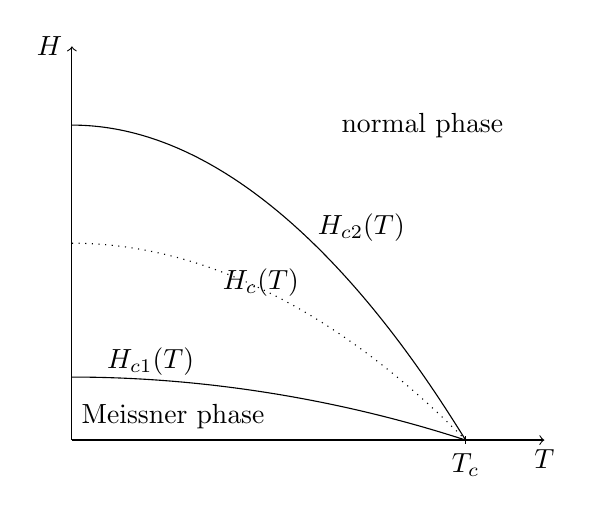
\begin{tikzpicture}
	\draw[->] (0,0)--(6,0) node[below]{$T$};
	\draw[->] (0,0)--(0,5) node[left]{$H$};

	\draw (0,0.8) parabola (5,0);
	\draw (0,4) parabola (5,0);
	\draw[dotted] (0,2.5) parabola (5,0);
	\draw (1,0.7) node[above]{$H_{c1}(T)$}
		(3, 2.7) node[right]{$H_{c2}(T)$}
		(2.4, 2.3) node[below]{$H_{c}(T)$}
		(0,0.3)node[right]{Meissner phase}
		(3.3,4)node[right]{normal phase};
	\draw (5,-0.05) node[below]{$T_c$} -- (5,0.05);
\end{tikzpicture}\\
Phase diagram of type-II superconductor
\end{center}
	\item Between $H_{c1}$ and $H_{c2}$ there's \textbf{``Abrikosov vortex
		lattice''}, partial flux expulsion of the field. 
		\begin{itemize}
		  \item one vortex per flux quantum
		  \item $\Phi_0 \approx \SI{20}{\gauss\micro\meter\squared}$ which
			  means \SI{100}{\angstrom} at \SI{20}{T} ($\gg$ atomic spacing) 
		\end{itemize}
	\item $H_{c1}$ is the transition of Meissner phase + 1 vortex line
		\begin{itemize}
			\item $|\Psi|$ below $\sqrt{|\alpha|/\beta}$ within
				$r\lesssim\xi$
			\item $\vec j$ increase within $r\lesssim\xi$ and decrease
				exponentially for $r\gg\lambda$
				\begin{equation}
					\mu_0H_{c1} \approx \frac{\Phi_0}{4\pi\lambda^2}\ln\kappa
				\end{equation}
		\end{itemize}
	\item Vortex motion $\Leftrightarrow$ voltage: if vortices can move,
		there's nonzero resistivity / Superconductivity only if vortices are
		immobile
	\item High-$H_{c2}$ material: ``pin'' the vortices using local
		impurities/defects that are less superconducting. 
	\item Thermal fluctuations of vortices in Abrikosov vortex lattice:
		melting transition from vortex solid(glass) to vortex liquid (resistive)
		\begin{itemize}
		  \item In vortex liquid $\langle\Psi\rangle = 0$ but $\langle
				  |\Psi|^2\rangle > 0$
		\end{itemize}
\end{itemize}

\section{2D electron systems and Quantum Hall effect}
\label{sec:2d_electron_systems_and_quantum_hall_effect}
\begin{itemize}
	\item Some effective mass (tensor, but assumed to be isotropic in the
		following), can be $m^* \ll m_e$
	\item Low density, spacing $\gg$ unit cells
\end{itemize}

\subsection{Integer Quantum Hall effect}
\label{sub:integer_quantum_hall_effect}
Add magnetic field: Landau levels and Zeeman splitting: 
\begin{equation}\label{eq:e_in_2d}
	\epsilon = \epsilon_0 + \hbar\omega_c \left\{ n+\frac 12 \right\} 
	+ g\mu_B \vec B\cdot\vec\sigma
\end{equation}
Note that the degeneracy of Landau level is one per flux quantum $j\le
\Phi/\Phi_0$, So the DOS is a sum of delta functions at $\hbar\omega_c ( n+
1/2)\pm g\mu_B |B|$, and the filling of states $\nu = \mbox{No. of
electrons}/\mbox{No. of flux quanta}$. 
\begin{itemize}
  \item $\nu\in\mathbb N$: Integer quantum Hall effect. Adding the potential
	  at edges, the band diagram: 
	  \begin{figure}[htpb]
	    \centering
	    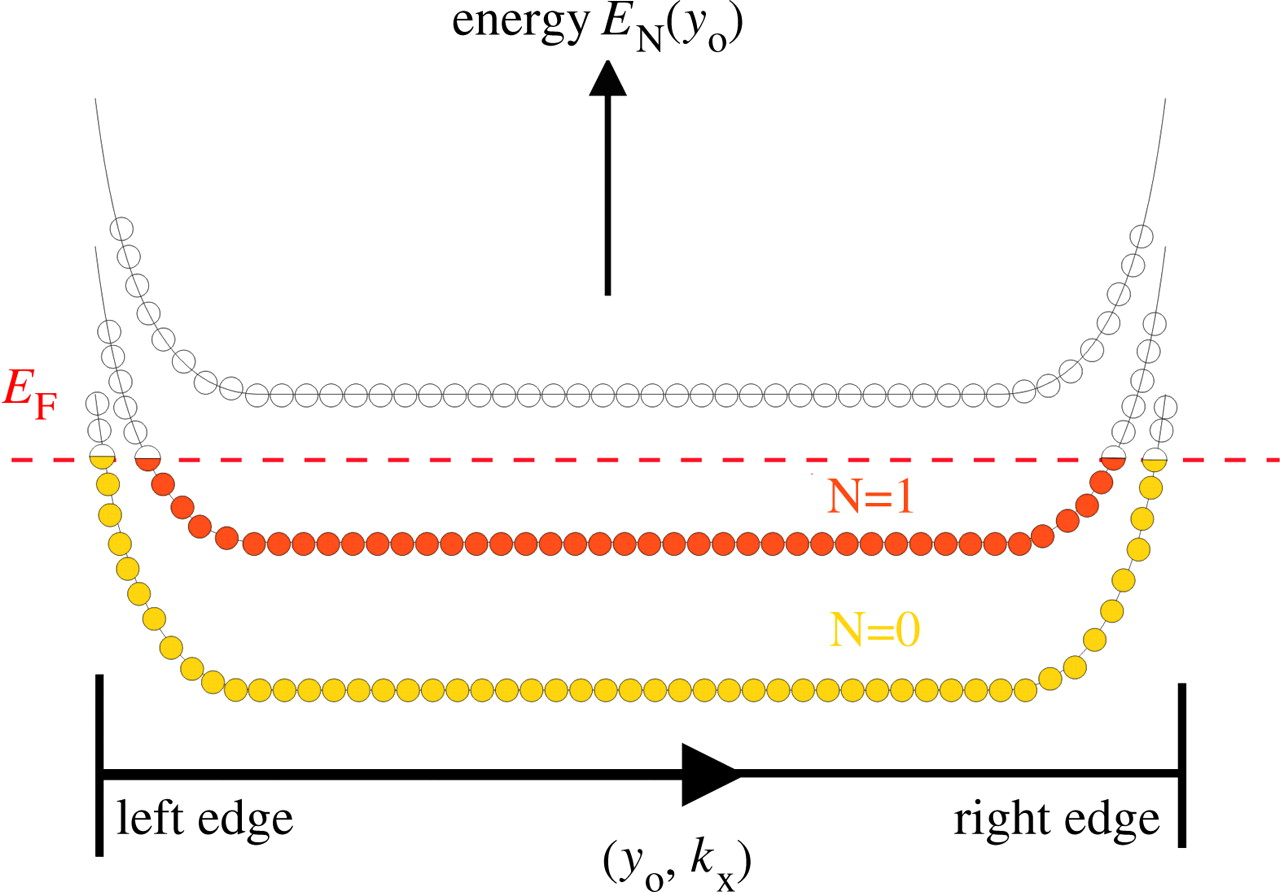
\includegraphics[width=0.6\linewidth]{integral_q_hall.jpg}
	  \end{figure}
	  \begin{itemize}
	    \item No gap with the edges, but states near $E_F$ are all at edges
		\item Edges of 2D integer quantum Hall system are 1D ``chiral metals"
		\item Gap in bulk (topological insulator), states at edge move only
			in one direction: $v_y = \dif\epsilon/\hbar\dif k_y$,
			$v_y>0$($<0$) at right(left) edge
		\item scattering from imperfections at edge does \emph{not} affect
			current, since all states have same direction of motion
		\item Net current in one Landau level: 
			\begin{equation}
				I_y = \frac{e}{2\pi}\int\dif k_y\, \frac 1\hbar
				\frac{\partial\epsilon}{\partial k_y} 
				= \frac eh \Delta \epsilon = \frac{e^2}{h}V_x
			\end{equation}
			which is robust to sample dimensions, disorder, weak
			interactions, but need to be at $T\ll \hbar\omega_c$.
			This now define the Ohm. 
	  \end{itemize}
\end{itemize}

\subsection{Wigner crystal of electrons}
\label{sub:wigner_crystal_of_electrons}
Add electron-electron interactions, but no $\vec B$. Coulomb potential and
kinetic energy compete: 
\begin{itemize}
  \item High density: kinetic energy ``wins'', it's a Fermi liquid
  \item Low density: \textbf{Wigner crystal}. Seen on electrons on helium
	  surface. 
  \item $\vec B\neq =$: kinetic energy drops out, but Landau level
	  $\hbar\omega_c$, and for low enough filling, \textbf{field-induced
	  Wigner crystal}. Seen in 2D semiconductors devices at low filling and
	  high field.
\end{itemize}

\subsection{Fractional quantum Hall effect}
\label{sub:fractional_quantum_hall_effect}
At high filling, such as $\nu = 1/5, 1/3, 2/5, 2/3...$, ground state is
\textbf{fractional quantum Hall effect}.

Under Coulomb gauge, the lowest Landau eigenfunctions are: 
\begin{equation}
	\Psi_m(z) = N_m z^m\e^{-|z|^2/4} = N_m r^m \e^{\mi m\phi}\e^{-|r|^2/4}
\end{equation}
Filled lowest Landau level wave function for $n$ electrons with anti-symmetry is: 
\begin{equation}
	\Psi^{(1)}(z_1, z_2, \cdots z_n) = N \left[ \prod_{i\neq j}^n (z_i-z_j)
	\right]\exp \left(-\sum_i \frac{|z_i|^2}{4}\right)
\end{equation}
which is called \textbf{``quantum Hall droplet''}. 

Laughlin(1983) gave wavefunction for filling $\nu=1/m$ with $m=1,2,3,...$
\begin{equation}
	\Psi^{(m)}(\{z_i\}) =  N \left[ \prod_{i\neq j}^n (z_i-z_j)^m
	\right]\exp \left(-\sum_i \frac{|z_i|^2}{4}\right)
\end{equation}
is exact eigenfunction in limit of short-range repulsion, and is very good
approximation for Coulomb.
\begin{itemize}
  \item For large $m$, low filling $\nu = 1/m$: Wigner crystal
  \item For $m=1,3,5,7$, Laughlin liquid of fractional quantum Hall effect:
	  fractional charged Laughlin quasi-particles. 
\end{itemize}

\end{document}
